\documentclass[twoside]{book}

% Packages required by doxygen
\usepackage{fixltx2e}
\usepackage{calc}
\usepackage{doxygen}
\usepackage[export]{adjustbox} % also loads graphicx
\usepackage{graphicx}
\usepackage[utf8]{inputenc}
\usepackage{makeidx}
\usepackage{multicol}
\usepackage{multirow}
\PassOptionsToPackage{warn}{textcomp}
\usepackage{textcomp}
\usepackage[nointegrals]{wasysym}
\usepackage[table]{xcolor}

% Font selection
\usepackage[T1]{fontenc}
\usepackage[scaled=.90]{helvet}
\usepackage{courier}
\usepackage{amssymb}
\usepackage{sectsty}
\renewcommand{\familydefault}{\sfdefault}
\allsectionsfont{%
  \fontseries{bc}\selectfont%
  \color{darkgray}%
}
\renewcommand{\DoxyLabelFont}{%
  \fontseries{bc}\selectfont%
  \color{darkgray}%
}
\newcommand{\+}{\discretionary{\mbox{\scriptsize$\hookleftarrow$}}{}{}}

% Page & text layout
\usepackage{geometry}
\geometry{%
  a4paper,%
  top=2.5cm,%
  bottom=2.5cm,%
  left=2.5cm,%
  right=2.5cm%
}
\tolerance=750
\hfuzz=15pt
\hbadness=750
\setlength{\emergencystretch}{15pt}
\setlength{\parindent}{0cm}
\setlength{\parskip}{3ex plus 2ex minus 2ex}
\makeatletter
\renewcommand{\paragraph}{%
  \@startsection{paragraph}{4}{0ex}{-1.0ex}{1.0ex}{%
    \normalfont\normalsize\bfseries\SS@parafont%
  }%
}
\renewcommand{\subparagraph}{%
  \@startsection{subparagraph}{5}{0ex}{-1.0ex}{1.0ex}{%
    \normalfont\normalsize\bfseries\SS@subparafont%
  }%
}
\makeatother

% Headers & footers
\usepackage{fancyhdr}
\pagestyle{fancyplain}
\fancyhead[LE]{\fancyplain{}{\bfseries\thepage}}
\fancyhead[CE]{\fancyplain{}{}}
\fancyhead[RE]{\fancyplain{}{\bfseries\leftmark}}
\fancyhead[LO]{\fancyplain{}{\bfseries\rightmark}}
\fancyhead[CO]{\fancyplain{}{}}
\fancyhead[RO]{\fancyplain{}{\bfseries\thepage}}
\fancyfoot[LE]{\fancyplain{}{}}
\fancyfoot[CE]{\fancyplain{}{}}
\fancyfoot[RE]{\fancyplain{}{\bfseries\scriptsize Generated by Doxygen }}
\fancyfoot[LO]{\fancyplain{}{\bfseries\scriptsize Generated by Doxygen }}
\fancyfoot[CO]{\fancyplain{}{}}
\fancyfoot[RO]{\fancyplain{}{}}
\renewcommand{\footrulewidth}{0.4pt}
\renewcommand{\chaptermark}[1]{%
  \markboth{#1}{}%
}
\renewcommand{\sectionmark}[1]{%
  \markright{\thesection\ #1}%
}

% Indices & bibliography
\usepackage{natbib}
\usepackage[titles]{tocloft}
\setcounter{tocdepth}{3}
\setcounter{secnumdepth}{5}
\makeindex

% Hyperlinks (required, but should be loaded last)
\usepackage{ifpdf}
\ifpdf
  \usepackage[pdftex,pagebackref=true]{hyperref}
\else
  \usepackage[ps2pdf,pagebackref=true]{hyperref}
\fi
\hypersetup{%
  colorlinks=true,%
  linkcolor=blue,%
  citecolor=blue,%
  unicode%
}

% Custom commands
\newcommand{\clearemptydoublepage}{%
  \newpage{\pagestyle{empty}\cleardoublepage}%
}

\usepackage{caption}
\captionsetup{labelsep=space,justification=centering,font={bf},singlelinecheck=off,skip=4pt,position=top}

%===== C O N T E N T S =====

\begin{document}

% Titlepage & ToC
\hypersetup{pageanchor=false,
             bookmarksnumbered=true,
             pdfencoding=unicode
            }
\pagenumbering{roman}
\begin{titlepage}
\vspace*{7cm}
\begin{center}%
{\Large My Project }\\
\vspace*{1cm}
{\large Generated by Doxygen 1.8.11}\\
\end{center}
\end{titlepage}
\clearemptydoublepage
\tableofcontents
\clearemptydoublepage
\pagenumbering{arabic}
\hypersetup{pageanchor=true}

%--- Begin generated contents ---
\chapter{Hierarchical Index}
\section{Class Hierarchy}
This inheritance list is sorted roughly, but not completely, alphabetically\+:\begin{DoxyCompactList}
\item \contentsline{section}{Case}{\pageref{class_case}}{}
\item \contentsline{section}{Damier}{\pageref{class_damier}}{}
\item \contentsline{section}{Piece}{\pageref{class_piece}}{}
\begin{DoxyCompactList}
\item \contentsline{section}{Fou}{\pageref{class_fou}}{}
\item \contentsline{section}{Knight}{\pageref{class_knight}}{}
\item \contentsline{section}{Pion}{\pageref{class_pion}}{}
\item \contentsline{section}{Reine}{\pageref{class_reine}}{}
\item \contentsline{section}{Roi}{\pageref{class_roi}}{}
\item \contentsline{section}{Tour}{\pageref{class_tour}}{}
\end{DoxyCompactList}
\item \contentsline{section}{Piece\+Img}{\pageref{class_piece_img}}{}
\item Application\begin{DoxyCompactList}
\item \contentsline{section}{Affichage}{\pageref{class_affichage}}{}
\item \contentsline{section}{Main}{\pageref{class_main}}{}
\end{DoxyCompactList}
\end{DoxyCompactList}

\chapter{Class Index}
\section{Class List}
Here are the classes, structs, unions and interfaces with brief descriptions\+:\begin{DoxyCompactList}
\item\contentsline{section}{\hyperlink{class_affichage}{Affichage} }{\pageref{class_affichage}}{}
\item\contentsline{section}{\hyperlink{class_case}{Case} }{\pageref{class_case}}{}
\item\contentsline{section}{\hyperlink{class_damier}{Damier} }{\pageref{class_damier}}{}
\item\contentsline{section}{\hyperlink{class_fou}{Fou} }{\pageref{class_fou}}{}
\item\contentsline{section}{\hyperlink{class_knight}{Knight} }{\pageref{class_knight}}{}
\item\contentsline{section}{\hyperlink{class_main}{Main} }{\pageref{class_main}}{}
\item\contentsline{section}{\hyperlink{class_piece}{Piece} }{\pageref{class_piece}}{}
\item\contentsline{section}{\hyperlink{class_piece_img}{Piece\+Img} }{\pageref{class_piece_img}}{}
\item\contentsline{section}{\hyperlink{class_pion}{Pion} }{\pageref{class_pion}}{}
\item\contentsline{section}{\hyperlink{class_reine}{Reine} }{\pageref{class_reine}}{}
\item\contentsline{section}{\hyperlink{class_roi}{Roi} }{\pageref{class_roi}}{}
\item\contentsline{section}{\hyperlink{class_tour}{Tour} }{\pageref{class_tour}}{}
\end{DoxyCompactList}

\chapter{Class Documentation}
\hypertarget{class_affichage}{}\section{Affichage Class Reference}
\label{class_affichage}\index{Affichage@{Affichage}}
Inheritance diagram for Affichage\+:\begin{figure}[H]
\begin{center}
\leavevmode
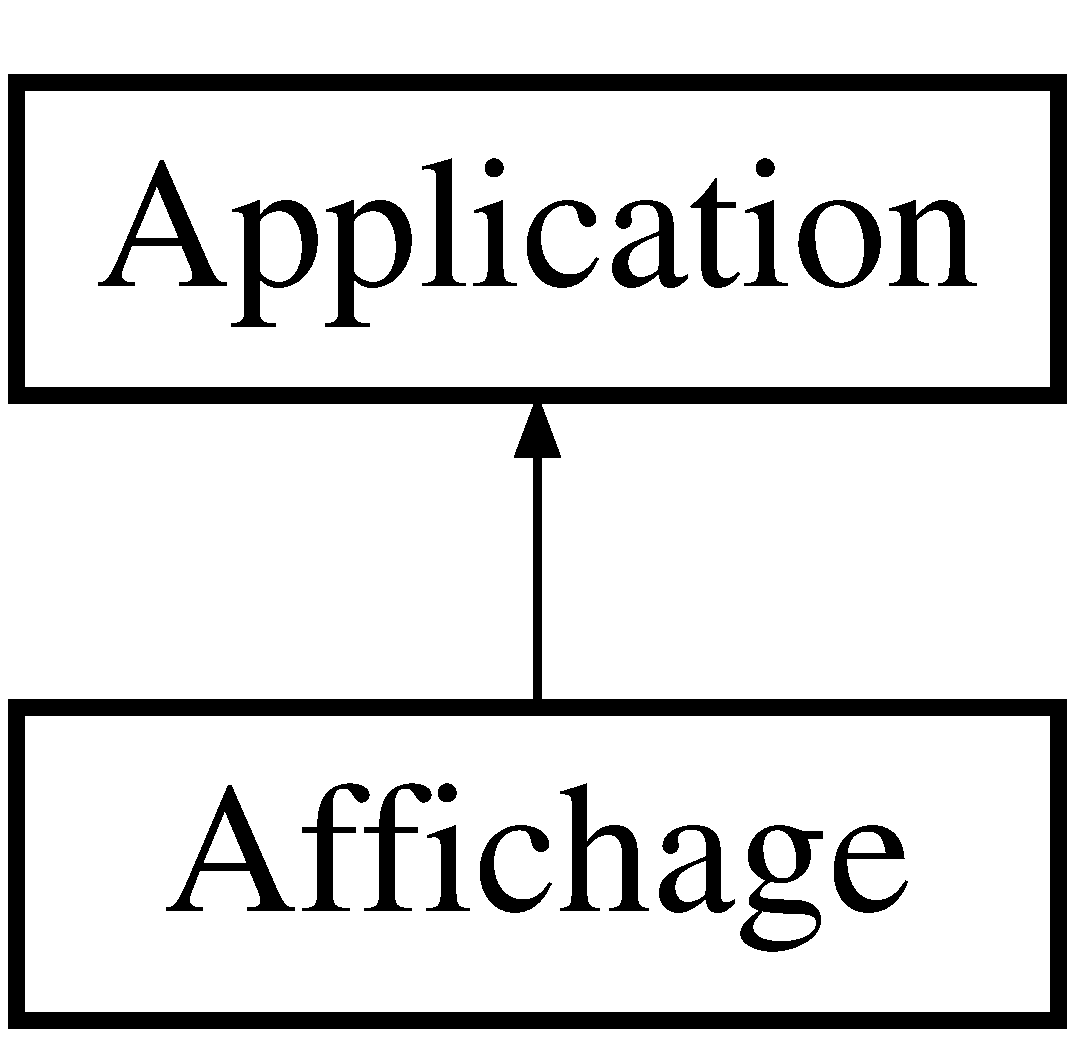
\includegraphics[height=2.000000cm]{class_affichage}
\end{center}
\end{figure}
\subsection*{Public Member Functions}
\begin{DoxyCompactItemize}
\item 
{\bfseries Affichage} (\hyperlink{class_damier}{Damier} damier)\hypertarget{class_affichage_a93128b3855e316b8e42c098f698a9b76}{}\label{class_affichage_a93128b3855e316b8e42c098f698a9b76}

\item 
void {\bfseries start} (Stage primary\+Stage)\hypertarget{class_affichage_a00681ef021675df896e280e8585b43f9}{}\label{class_affichage_a00681ef021675df896e280e8585b43f9}

\item 
void {\bfseries main} (String\mbox{[}$\,$\mbox{]} args)\hypertarget{class_affichage_abcbe888db7858bdcea3d1476cea127db}{}\label{class_affichage_abcbe888db7858bdcea3d1476cea127db}

\end{DoxyCompactItemize}


The documentation for this class was generated from the following file\+:\begin{DoxyCompactItemize}
\item 
Affichage.\+java\end{DoxyCompactItemize}

\hypertarget{class_case}{}\section{Case Class Reference}
\label{class_case}\index{Case@{Case}}
\subsection*{Public Member Functions}
\begin{DoxyCompactItemize}
\item 
{\bfseries Case} (int x, int y, \hyperlink{class_damier}{Damier} damier)\hypertarget{class_case_ae64d387de91dc66844e607afeeeec911}{}\label{class_case_ae64d387de91dc66844e607afeeeec911}

\item 
int {\bfseries getX} ()\hypertarget{class_case_a809c70632df92bf71504afe2c3401be4}{}\label{class_case_a809c70632df92bf71504afe2c3401be4}

\item 
int {\bfseries getY} ()\hypertarget{class_case_a382d788769c0ee8c984ed47b8a24585d}{}\label{class_case_a382d788769c0ee8c984ed47b8a24585d}

\item 
\hyperlink{class_piece}{Piece} {\bfseries get\+Piece} ()\hypertarget{class_case_a642391cf4cff2ec20ebc8909ecbb562d}{}\label{class_case_a642391cf4cff2ec20ebc8909ecbb562d}

\item 
\hyperlink{class_damier}{Damier} {\bfseries get\+Damier} ()\hypertarget{class_case_afe8c3c5323166c31d7c758dbc2efd080}{}\label{class_case_afe8c3c5323166c31d7c758dbc2efd080}

\item 
void {\bfseries setX} (int x)\hypertarget{class_case_ac46e99e107e16075b1cf4b14066e50af}{}\label{class_case_ac46e99e107e16075b1cf4b14066e50af}

\item 
void {\bfseries setY} (int y)\hypertarget{class_case_a704d56ebbeb2a8cd500a361090c152f3}{}\label{class_case_a704d56ebbeb2a8cd500a361090c152f3}

\item 
void {\bfseries set\+Piece} (\hyperlink{class_piece}{Piece} piece)\hypertarget{class_case_a1b222c7d71df614c4a0899c80babe196}{}\label{class_case_a1b222c7d71df614c4a0899c80babe196}

\item 
void {\bfseries set\+Damier} (\hyperlink{class_damier}{Damier} damier)\hypertarget{class_case_a6db0b310d4eaf0ae984b9f489c4ccf4b}{}\label{class_case_a6db0b310d4eaf0ae984b9f489c4ccf4b}

\item 
\hyperlink{class_case}{Case} {\bfseries copie\+Case} ()\hypertarget{class_case_af0f47703c89d8337c4b5839bf2dc12cd}{}\label{class_case_af0f47703c89d8337c4b5839bf2dc12cd}

\item 
boolean {\bfseries equal} (\hyperlink{class_case}{Case} yop)\hypertarget{class_case_a371c658843374088f839c2ed567f0fc8}{}\label{class_case_a371c658843374088f839c2ed567f0fc8}

\end{DoxyCompactItemize}


\subsection{Detailed Description}
\begin{DoxyAuthor}{Author}
Pierrick 
\end{DoxyAuthor}


The documentation for this class was generated from the following file\+:\begin{DoxyCompactItemize}
\item 
Case.\+java\end{DoxyCompactItemize}

\hypertarget{class_damier}{}\section{Damier Class Reference}
\label{class_damier}\index{Damier@{Damier}}
\subsection*{Public Member Functions}
\begin{DoxyCompactItemize}
\item 
\hyperlink{class_case}{Case} {\bfseries get\+Case} (int x, int y)\hypertarget{class_damier_a8103d1111efad33bf34d96776c69da8b}{}\label{class_damier_a8103d1111efad33bf34d96776c69da8b}

\item 
void {\bfseries set\+Case} (int x, int y, \hyperlink{class_case}{Case} yop)\hypertarget{class_damier_a55fe727de5bca3f52824306b5a346bee}{}\label{class_damier_a55fe727de5bca3f52824306b5a346bee}

\item 
\hyperlink{class_damier}{Damier} {\bfseries copie\+Damier} ()\hypertarget{class_damier_a8b0caf22e0988e8f9ea8ded7929f856f}{}\label{class_damier_a8b0caf22e0988e8f9ea8ded7929f856f}

\item 
void {\bfseries initialiser} ()\hypertarget{class_damier_a3d6f1e06e2626618397cc6fbec2a588b}{}\label{class_damier_a3d6f1e06e2626618397cc6fbec2a588b}

\item 
void {\bfseries deplacer} (\hyperlink{class_case}{Case} depart, \hyperlink{class_case}{Case} arrivee)\hypertarget{class_damier_a6abc997fa2c561dd41d721c9752a4804}{}\label{class_damier_a6abc997fa2c561dd41d721c9752a4804}

\item 
void {\bfseries manger} (\hyperlink{class_case}{Case} yop)\hypertarget{class_damier_ad11d7a281b1f3beb869710e24a275c12}{}\label{class_damier_ad11d7a281b1f3beb869710e24a275c12}

\item 
\hyperlink{class_case}{Case} {\bfseries Nord} (\hyperlink{class_case}{Case} yop)\hypertarget{class_damier_ab0eabeab7fcfa1c1e43e8a696f3b82e6}{}\label{class_damier_ab0eabeab7fcfa1c1e43e8a696f3b82e6}

\item 
\hyperlink{class_case}{Case} {\bfseries Sud} (\hyperlink{class_case}{Case} yop)\hypertarget{class_damier_a78ff2eb41c02ec2f6e68219746e38219}{}\label{class_damier_a78ff2eb41c02ec2f6e68219746e38219}

\item 
\hyperlink{class_case}{Case} {\bfseries Ouest} (\hyperlink{class_case}{Case} yop)\hypertarget{class_damier_ab7ee970b51b4c0226ffd818ee7b25f4f}{}\label{class_damier_ab7ee970b51b4c0226ffd818ee7b25f4f}

\item 
\hyperlink{class_case}{Case} {\bfseries Est} (\hyperlink{class_case}{Case} yop)\hypertarget{class_damier_a3347285ddc8bd1def8d393ddcb3ef68d}{}\label{class_damier_a3347285ddc8bd1def8d393ddcb3ef68d}

\item 
\hyperlink{class_case}{Case} {\bfseries NW} (\hyperlink{class_case}{Case} yop)\hypertarget{class_damier_a44ecf6c5e0d0ac651e36568a83a8dd90}{}\label{class_damier_a44ecf6c5e0d0ac651e36568a83a8dd90}

\item 
\hyperlink{class_case}{Case} {\bfseries NE} (\hyperlink{class_case}{Case} yop)\hypertarget{class_damier_afba7ae9ce0ca580b6803ceae326f5e02}{}\label{class_damier_afba7ae9ce0ca580b6803ceae326f5e02}

\item 
\hyperlink{class_case}{Case} {\bfseries SW} (\hyperlink{class_case}{Case} yop)\hypertarget{class_damier_ad317036c71ddb0eaabcf8b754c70e37e}{}\label{class_damier_ad317036c71ddb0eaabcf8b754c70e37e}

\item 
\hyperlink{class_case}{Case} {\bfseries SE} (\hyperlink{class_case}{Case} yop)\hypertarget{class_damier_aa310ab704cc37cb5c1ef8953012ae9c8}{}\label{class_damier_aa310ab704cc37cb5c1ef8953012ae9c8}

\item 
boolean {\bfseries action\+Possible} (\hyperlink{class_case}{Case} yop, int joueur)\hypertarget{class_damier_ab15b6599529770e83b70936e89e69235}{}\label{class_damier_ab15b6599529770e83b70936e89e69235}

\item 
boolean {\bfseries deplacement\+Possible} (\hyperlink{class_case}{Case} depart, \hyperlink{class_case}{Case} arrivee, int joueur)\hypertarget{class_damier_ace56252a058aa7c8ca7ed5f36699d10d}{}\label{class_damier_ace56252a058aa7c8ca7ed5f36699d10d}

\item 
\hyperlink{class_case}{Case} {\bfseries attaque\+Possible} (\hyperlink{class_case}{Case} depart, \hyperlink{class_case}{Case} arrivee, int joueur)\hypertarget{class_damier_aa55a611ac55d1fd9af10d231aa63bfb4}{}\label{class_damier_aa55a611ac55d1fd9af10d231aa63bfb4}

\item 
boolean {\bfseries is\+Attaque\+Possible} (\hyperlink{class_case}{Case} yop, int joueur)\hypertarget{class_damier_a28e1257dd6bed520d005a0eed97111f3}{}\label{class_damier_a28e1257dd6bed520d005a0eed97111f3}

\item 
Array\+List$<$ \hyperlink{class_case}{Case} $>$ {\bfseries all\+Pions} (int joueur)\hypertarget{class_damier_acc78f205170c7862ebb453db663ccb1e}{}\label{class_damier_acc78f205170c7862ebb453db663ccb1e}

\item 
Array\+List$<$ \hyperlink{class_case}{Case} $>$ {\bfseries is\+Attaquepossible\+Somewhere} (int joueur)\hypertarget{class_damier_a4b6ed4ba50b7d3ed5a4a880e7f9a256b}{}\label{class_damier_a4b6ed4ba50b7d3ed5a4a880e7f9a256b}

\end{DoxyCompactItemize}


\subsection{Detailed Description}
\begin{DoxyAuthor}{Author}
Pierrick 
\end{DoxyAuthor}


The documentation for this class was generated from the following file\+:\begin{DoxyCompactItemize}
\item 
Damier.\+java\end{DoxyCompactItemize}

\hypertarget{class_fou}{}\section{Fou Class Reference}
\label{class_fou}\index{Fou@{Fou}}
Inheritance diagram for Fou\+:\begin{figure}[H]
\begin{center}
\leavevmode
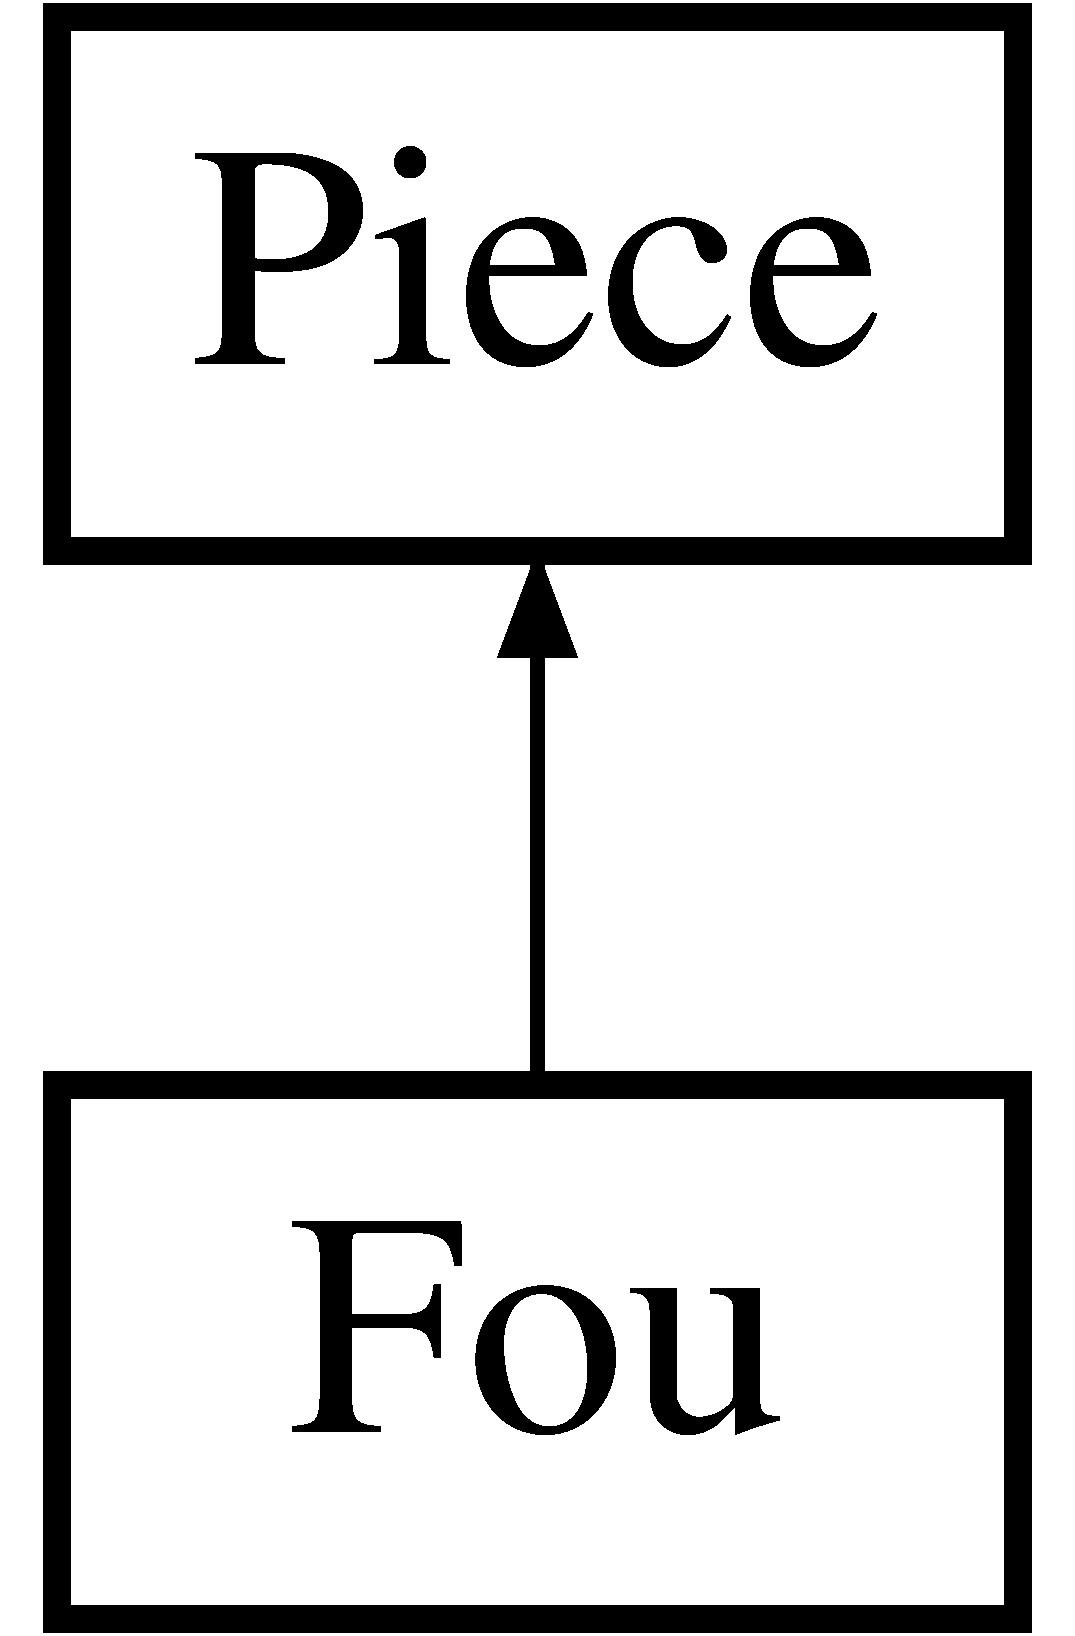
\includegraphics[height=2.000000cm]{class_fou}
\end{center}
\end{figure}
\subsection*{Public Member Functions}
\begin{DoxyCompactItemize}
\item 
{\bfseries Fou} (\hyperlink{class_case}{Case} yop)\hypertarget{class_fou_a37d926b3270c1de7f82fae34c95b4277}{}\label{class_fou_a37d926b3270c1de7f82fae34c95b4277}

\item 
{\bfseries Fou} (int couleur, \hyperlink{class_case}{Case} yop)\hypertarget{class_fou_ac287e82db0fa269820953dfb6fd6a906}{}\label{class_fou_ac287e82db0fa269820953dfb6fd6a906}

\item 
Array\+List$<$ \hyperlink{class_case}{Case} $>$ {\bfseries cases\+Disponibles} ()\hypertarget{class_fou_a9c31eafd2fb1a30d9c36bbe4e6a4e35f}{}\label{class_fou_a9c31eafd2fb1a30d9c36bbe4e6a4e35f}

\end{DoxyCompactItemize}
\subsection*{Additional Inherited Members}


The documentation for this class was generated from the following file\+:\begin{DoxyCompactItemize}
\item 
Fou.\+java\end{DoxyCompactItemize}

\hypertarget{class_knight}{}\section{Knight Class Reference}
\label{class_knight}\index{Knight@{Knight}}
Inheritance diagram for Knight\+:\begin{figure}[H]
\begin{center}
\leavevmode
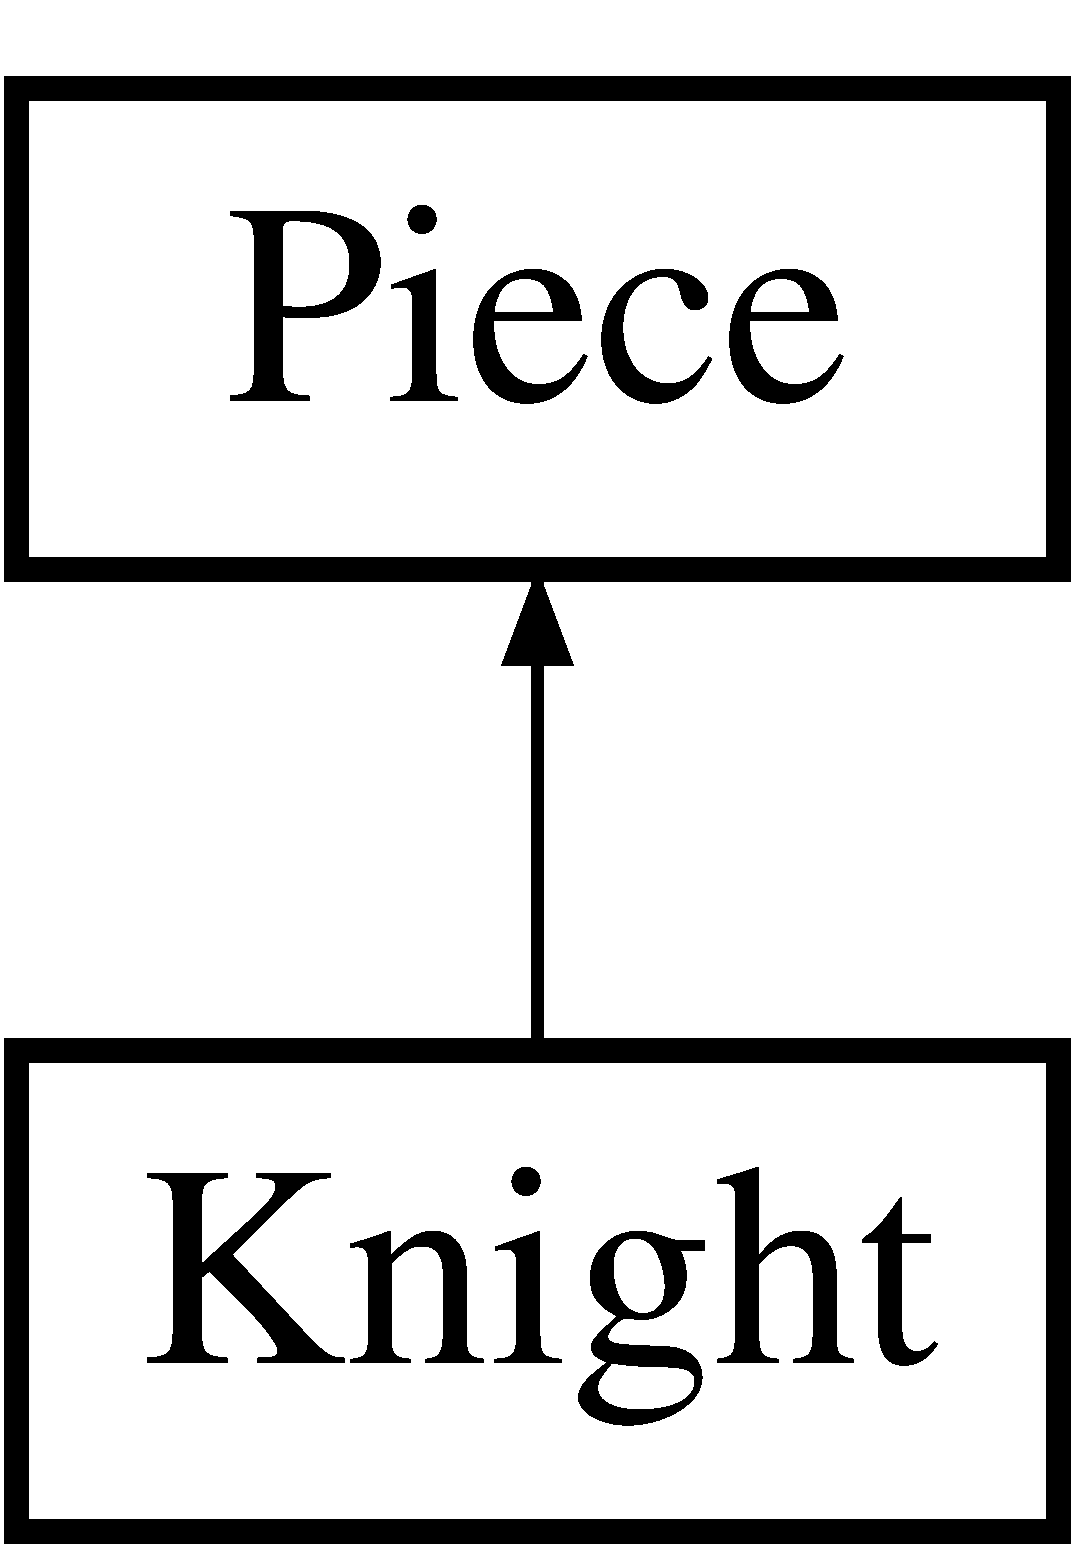
\includegraphics[height=2.000000cm]{class_knight}
\end{center}
\end{figure}
\subsection*{Public Member Functions}
\begin{DoxyCompactItemize}
\item 
{\bfseries Knight} (\hyperlink{class_case}{Case} yop)\hypertarget{class_knight_a6e7b3f713650528950fd360c9b1b338a}{}\label{class_knight_a6e7b3f713650528950fd360c9b1b338a}

\item 
{\bfseries Knight} (int couleur, \hyperlink{class_case}{Case} yop)\hypertarget{class_knight_afee7a5f9bcb1ee7029b5e0e8415c14c9}{}\label{class_knight_afee7a5f9bcb1ee7029b5e0e8415c14c9}

\item 
Array\+List$<$ \hyperlink{class_case}{Case} $>$ {\bfseries cases\+Disponibles} ()\hypertarget{class_knight_a017b56f82bf9cee77a16c9f3e1f1e24d}{}\label{class_knight_a017b56f82bf9cee77a16c9f3e1f1e24d}

\end{DoxyCompactItemize}
\subsection*{Additional Inherited Members}


\subsection{Detailed Description}
\begin{DoxyAuthor}{Author}
Pierrick 
\end{DoxyAuthor}


The documentation for this class was generated from the following file\+:\begin{DoxyCompactItemize}
\item 
Knight.\+java\end{DoxyCompactItemize}

\hypertarget{class_main}{}\section{Main Class Reference}
\label{class_main}\index{Main@{Main}}
Inheritance diagram for Main\+:\begin{figure}[H]
\begin{center}
\leavevmode
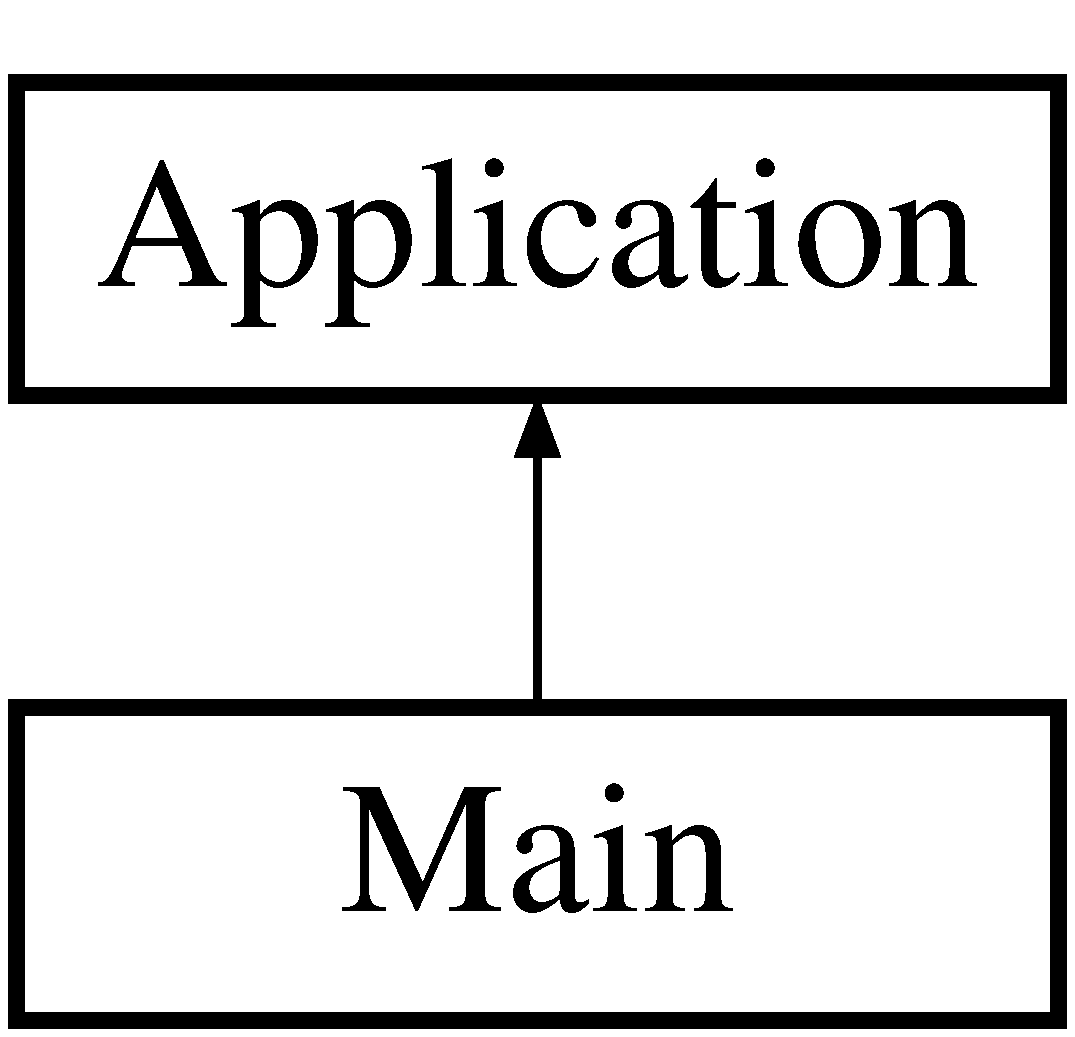
\includegraphics[height=2.000000cm]{class_main}
\end{center}
\end{figure}
\subsection*{Public Member Functions}
\begin{DoxyCompactItemize}
\item 
void {\bfseries start} (Stage primary\+Stage)  throws Exception \hypertarget{class_main_aaa75b38812324d0f17c89f139bde6ada}{}\label{class_main_aaa75b38812324d0f17c89f139bde6ada}

\end{DoxyCompactItemize}
\subsection*{Static Public Member Functions}
\begin{DoxyCompactItemize}
\item 
static void \hyperlink{class_main_a8a5d0f827edddff706cc0e6740d0579a}{main} (String\mbox{[}$\,$\mbox{]} args)
\end{DoxyCompactItemize}


\subsection{Member Function Documentation}
\index{Main@{Main}!main@{main}}
\index{main@{main}!Main@{Main}}
\subsubsection[{\texorpdfstring{main(\+String[] args)}{main(String[] args)}}]{\setlength{\rightskip}{0pt plus 5cm}static void Main.\+main (
\begin{DoxyParamCaption}
\item[{String\mbox{[}$\,$\mbox{]}}]{args}
\end{DoxyParamCaption}
)\hspace{0.3cm}{\ttfamily [inline]}, {\ttfamily [static]}}\hypertarget{class_main_a8a5d0f827edddff706cc0e6740d0579a}{}\label{class_main_a8a5d0f827edddff706cc0e6740d0579a}

\begin{DoxyParams}{Parameters}
{\em args} & \\
\hline
\end{DoxyParams}


The documentation for this class was generated from the following file\+:\begin{DoxyCompactItemize}
\item 
Main.\+java\end{DoxyCompactItemize}

\hypertarget{class_piece}{}\section{Piece Class Reference}
\label{class_piece}\index{Piece@{Piece}}
Inheritance diagram for Piece\+:\begin{figure}[H]
\begin{center}
\leavevmode
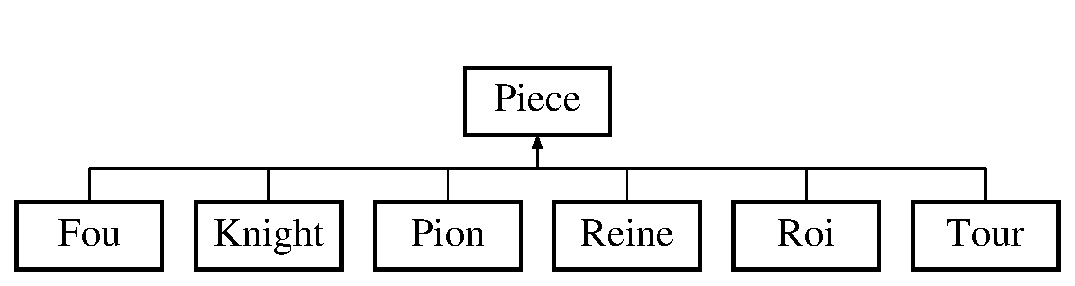
\includegraphics[height=2.000000cm]{class_piece}
\end{center}
\end{figure}
\subsection*{Public Member Functions}
\begin{DoxyCompactItemize}
\item 
{\bfseries Piece} (\hyperlink{class_case}{Case} yop)\hypertarget{class_piece_adf0013bc165221b7bc22fd2e57f0ff86}{}\label{class_piece_adf0013bc165221b7bc22fd2e57f0ff86}

\item 
{\bfseries Piece} (int couleur, \hyperlink{class_case}{Case} yop)\hypertarget{class_piece_ad578f789bad2e383f2fd2af092e8adfd}{}\label{class_piece_ad578f789bad2e383f2fd2af092e8adfd}

\item 
int {\bfseries get\+Couleur} ()\hypertarget{class_piece_a6abb7c0a71b21d4caab617d41010f74c}{}\label{class_piece_a6abb7c0a71b21d4caab617d41010f74c}

\item 
void {\bfseries set\+Couleur} (int couleur)\hypertarget{class_piece_acf8e906bed19768f54bb7d108d8695c1}{}\label{class_piece_acf8e906bed19768f54bb7d108d8695c1}

\item 
\hyperlink{class_case}{Case} {\bfseries get\+Case} ()\hypertarget{class_piece_a2e6564dbdd3d2768c4729ce889e1a773}{}\label{class_piece_a2e6564dbdd3d2768c4729ce889e1a773}

\item 
void {\bfseries set\+Case} (\hyperlink{class_case}{Case} yop)\hypertarget{class_piece_ab9f592cc87fcc10dd4bcf2ec69d5d85e}{}\label{class_piece_ab9f592cc87fcc10dd4bcf2ec69d5d85e}

\item 
String {\bfseries get\+Nom} ()\hypertarget{class_piece_aacd6bc2cee1f8ca7e5cd71f9be0b563b}{}\label{class_piece_aacd6bc2cee1f8ca7e5cd71f9be0b563b}

\item 
void {\bfseries set\+Nom} (String nom)\hypertarget{class_piece_ae3867c35f04f29ae99362b20c942f2ac}{}\label{class_piece_ae3867c35f04f29ae99362b20c942f2ac}

\item 
Image\+View {\bfseries get\+Img\+View} ()\hypertarget{class_piece_a90e24233543416fe6e8b57afa60df0f8}{}\label{class_piece_a90e24233543416fe6e8b57afa60df0f8}

\item 
void {\bfseries set\+Img\+View} (Image\+View pi)\hypertarget{class_piece_a12ce1a949c9a0f427333320392e54ce8}{}\label{class_piece_a12ce1a949c9a0f427333320392e54ce8}

\item 
\hyperlink{class_piece}{Piece} {\bfseries copie\+Piece} ()\hypertarget{class_piece_a181452ee8085960571073800459927b2}{}\label{class_piece_a181452ee8085960571073800459927b2}

\item 
boolean {\bfseries equal} (\hyperlink{class_piece}{Piece} piece)\hypertarget{class_piece_a7f9f2a3c7eda5a514b4170a354a85219}{}\label{class_piece_a7f9f2a3c7eda5a514b4170a354a85219}

\item 
Array\+List$<$ \hyperlink{class_case}{Case} $>$ {\bfseries cases\+Disponibles} ()\hypertarget{class_piece_a4023e5d15a349d33a4751de3715f8fd5}{}\label{class_piece_a4023e5d15a349d33a4751de3715f8fd5}

\item 
\hyperlink{class_piece}{Piece} {\bfseries Nord} ()\hypertarget{class_piece_a3632015f5d1331181681bb66ccd4bfb9}{}\label{class_piece_a3632015f5d1331181681bb66ccd4bfb9}

\item 
\hyperlink{class_piece}{Piece} {\bfseries Sud} ()\hypertarget{class_piece_a29bbc81f7f3590113cbc8bb0f5b93f28}{}\label{class_piece_a29bbc81f7f3590113cbc8bb0f5b93f28}

\item 
\hyperlink{class_piece}{Piece} {\bfseries Ouest} ()\hypertarget{class_piece_a214faa1a1483788ef65dc508f754be61}{}\label{class_piece_a214faa1a1483788ef65dc508f754be61}

\item 
\hyperlink{class_piece}{Piece} {\bfseries Est} ()\hypertarget{class_piece_ae70dd25fc57b4db1e2e5dee0f2771a25}{}\label{class_piece_ae70dd25fc57b4db1e2e5dee0f2771a25}

\item 
\hyperlink{class_piece}{Piece} {\bfseries NW} ()\hypertarget{class_piece_ae6ca403a299e7eac82168442dd652b28}{}\label{class_piece_ae6ca403a299e7eac82168442dd652b28}

\item 
\hyperlink{class_piece}{Piece} {\bfseries NE} ()\hypertarget{class_piece_af23d8d7f49b2da14f7c618b9966175f9}{}\label{class_piece_af23d8d7f49b2da14f7c618b9966175f9}

\item 
\hyperlink{class_piece}{Piece} {\bfseries SW} ()\hypertarget{class_piece_a6d1f8de619898cd2e29c394a4d8eecc0}{}\label{class_piece_a6d1f8de619898cd2e29c394a4d8eecc0}

\item 
\hyperlink{class_piece}{Piece} {\bfseries SE} ()\hypertarget{class_piece_af3553cdbbfa760fb29b5e83bbeb80d2c}{}\label{class_piece_af3553cdbbfa760fb29b5e83bbeb80d2c}

\item 
int {\bfseries is\+Allie} (\hyperlink{class_piece}{Piece} piece)\hypertarget{class_piece_aa6d5305cf852ce3aee36198e5f83e29a}{}\label{class_piece_aa6d5305cf852ce3aee36198e5f83e29a}

\end{DoxyCompactItemize}
\subsection*{Public Attributes}
\begin{DoxyCompactItemize}
\item 
int {\bfseries couleur}\hypertarget{class_piece_ad20c514044b4f915f6632e16a6650481}{}\label{class_piece_ad20c514044b4f915f6632e16a6650481}

\item 
\hyperlink{class_case}{Case} {\bfseries yop}\hypertarget{class_piece_ab50473158b8d3fcba018f3a759d335f5}{}\label{class_piece_ab50473158b8d3fcba018f3a759d335f5}

\item 
String {\bfseries nom}\hypertarget{class_piece_ac45bccda0ddc8fba99cbfcdc1e2d252b}{}\label{class_piece_ac45bccda0ddc8fba99cbfcdc1e2d252b}

\item 
\hyperlink{class_piece_img}{Piece\+Img} {\bfseries pi}\hypertarget{class_piece_a62067ca330d854d5b75fdb85c7628c76}{}\label{class_piece_a62067ca330d854d5b75fdb85c7628c76}

\end{DoxyCompactItemize}


\subsection{Detailed Description}
\begin{DoxyAuthor}{Author}
Pierrick 
\end{DoxyAuthor}


The documentation for this class was generated from the following file\+:\begin{DoxyCompactItemize}
\item 
Piece.\+java\end{DoxyCompactItemize}

\hypertarget{class_piece_img}{}\section{Piece\+Img Class Reference}
\label{class_piece_img}\index{Piece\+Img@{Piece\+Img}}
\subsection*{Public Member Functions}
\begin{DoxyCompactItemize}
\item 
{\bfseries Piece\+Img} (int i, boolean noir)\hypertarget{class_piece_img_a774ff3b1c3d8ffaf3ade7299b3229054}{}\label{class_piece_img_a774ff3b1c3d8ffaf3ade7299b3229054}

\end{DoxyCompactItemize}


The documentation for this class was generated from the following file\+:\begin{DoxyCompactItemize}
\item 
Piece\+Img.\+java\end{DoxyCompactItemize}

\hypertarget{class_pion}{}\section{Pion Class Reference}
\label{class_pion}\index{Pion@{Pion}}
Inheritance diagram for Pion\+:\begin{figure}[H]
\begin{center}
\leavevmode
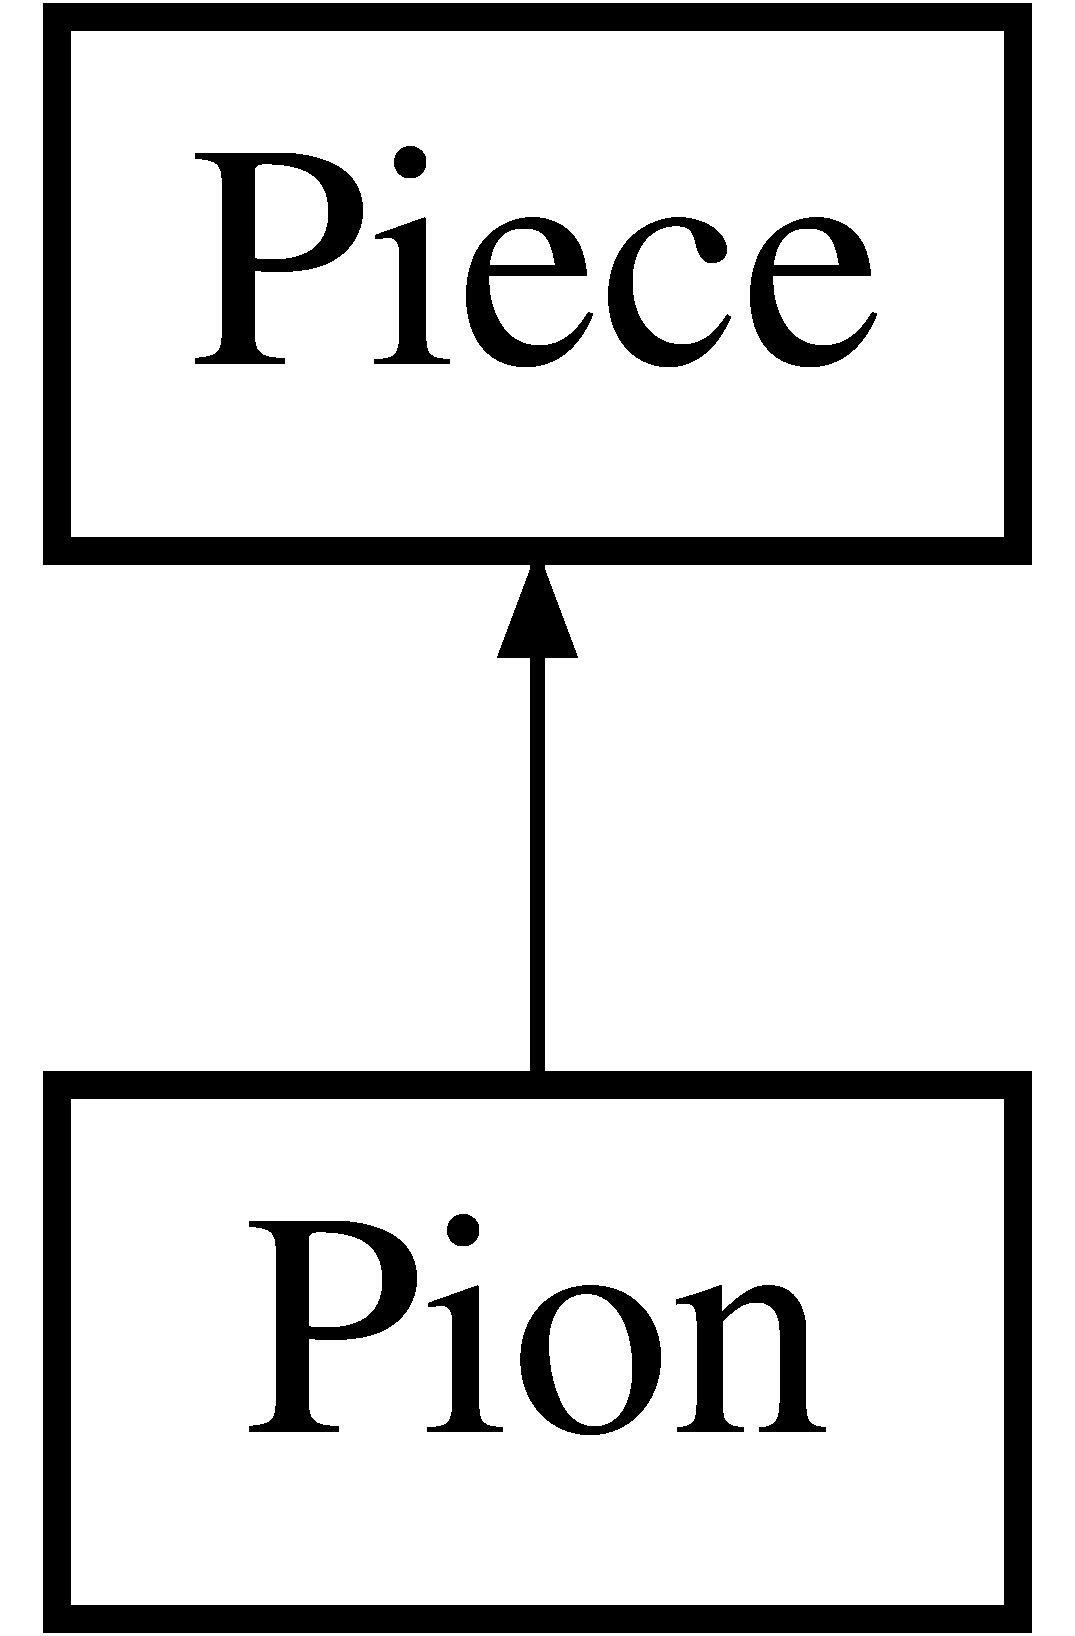
\includegraphics[height=2.000000cm]{class_pion}
\end{center}
\end{figure}
\subsection*{Public Member Functions}
\begin{DoxyCompactItemize}
\item 
{\bfseries Pion} (\hyperlink{class_case}{Case} yop)\hypertarget{class_pion_a500086d10acd8c4d0cae02a81a1dee9c}{}\label{class_pion_a500086d10acd8c4d0cae02a81a1dee9c}

\item 
{\bfseries Pion} (int couleur, \hyperlink{class_case}{Case} yop)\hypertarget{class_pion_a3b34db5e4efb2685cdc20b56bbdc8f39}{}\label{class_pion_a3b34db5e4efb2685cdc20b56bbdc8f39}

\item 
void {\bfseries conversion} (\hyperlink{class_pion}{Pion} timalchris)\hypertarget{class_pion_a7fd483c15bbdcc0ccba1dc2d45700756}{}\label{class_pion_a7fd483c15bbdcc0ccba1dc2d45700756}

\item 
Array\+List$<$ \hyperlink{class_case}{Case} $>$ {\bfseries cases\+Disponibles} ()\hypertarget{class_pion_ac523e0b691274788dc3914ad62ea0f49}{}\label{class_pion_ac523e0b691274788dc3914ad62ea0f49}

\end{DoxyCompactItemize}
\subsection*{Additional Inherited Members}


\subsection{Detailed Description}
\begin{DoxyAuthor}{Author}
Pierrick 
\end{DoxyAuthor}


The documentation for this class was generated from the following file\+:\begin{DoxyCompactItemize}
\item 
Pion.\+java\end{DoxyCompactItemize}

\hypertarget{class_reine}{}\section{Reine Class Reference}
\label{class_reine}\index{Reine@{Reine}}
Inheritance diagram for Reine\+:\begin{figure}[H]
\begin{center}
\leavevmode
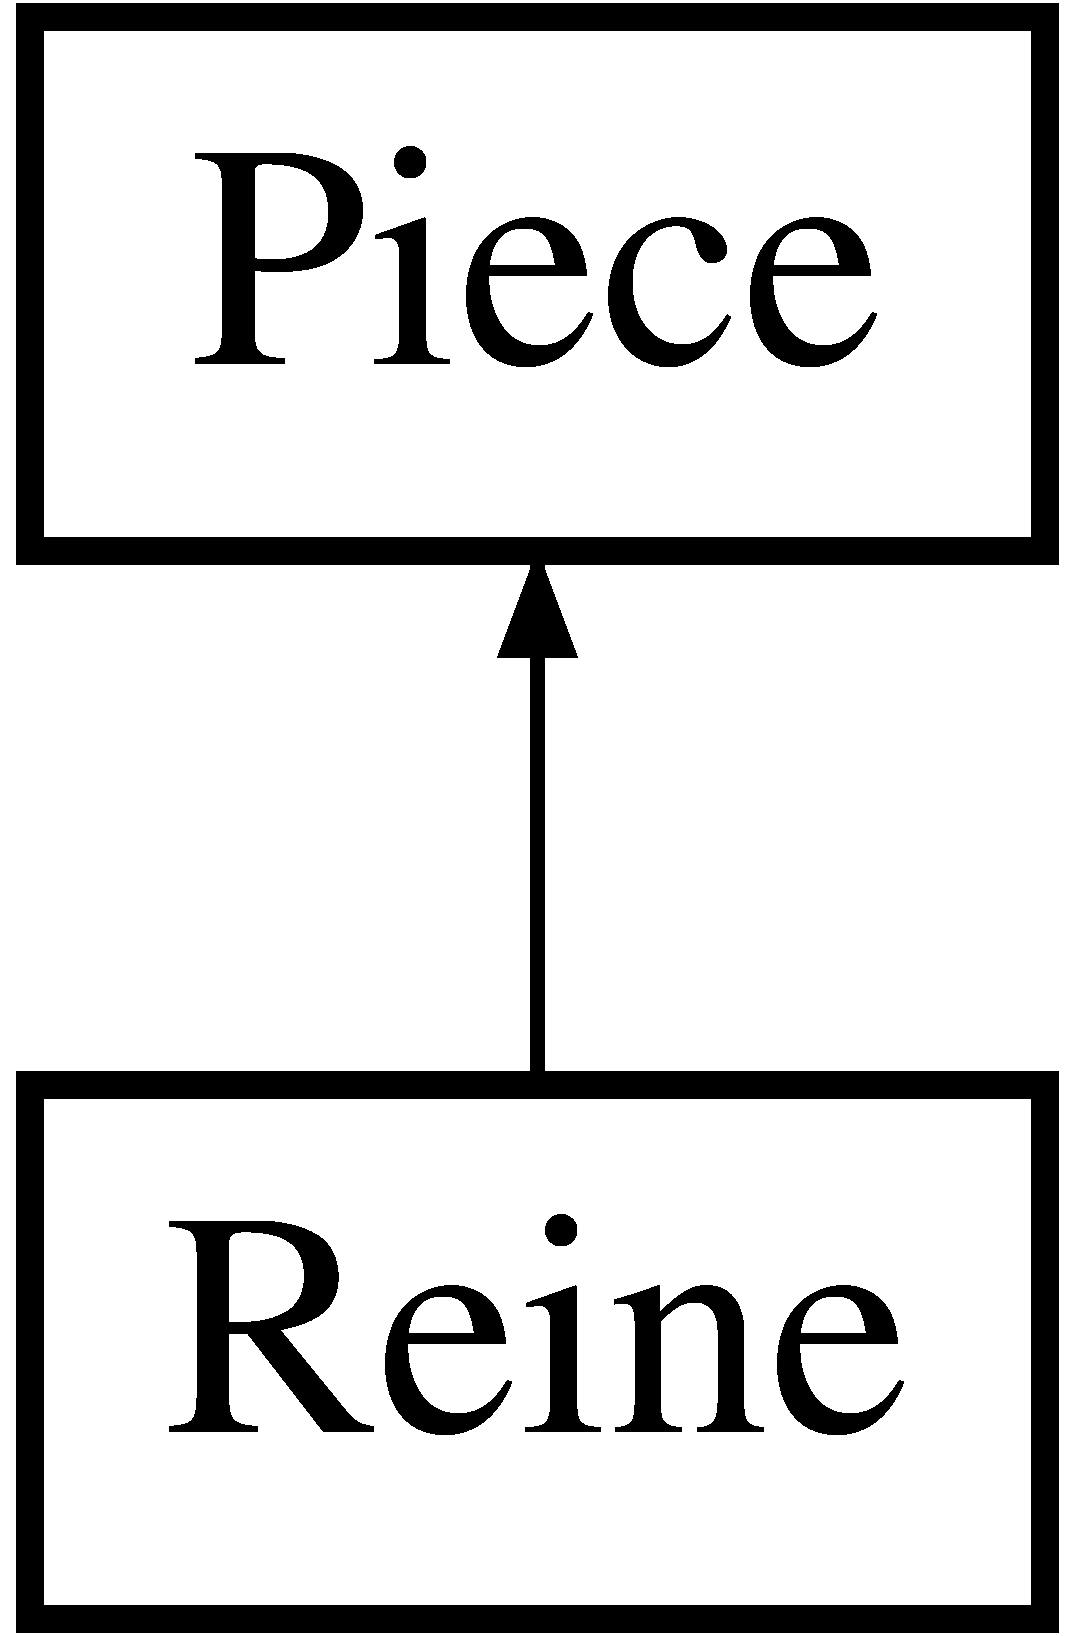
\includegraphics[height=2.000000cm]{class_reine}
\end{center}
\end{figure}
\subsection*{Public Member Functions}
\begin{DoxyCompactItemize}
\item 
{\bfseries Reine} (\hyperlink{class_case}{Case} yop)\hypertarget{class_reine_abba411a6ba9559a831382cc4eee14afc}{}\label{class_reine_abba411a6ba9559a831382cc4eee14afc}

\item 
{\bfseries Reine} (int couleur, \hyperlink{class_case}{Case} yop)\hypertarget{class_reine_ae5d6a09e7c2df6dd38ff96a062ed25aa}{}\label{class_reine_ae5d6a09e7c2df6dd38ff96a062ed25aa}

\item 
Array\+List$<$ \hyperlink{class_case}{Case} $>$ {\bfseries cases\+Disponibles} ()\hypertarget{class_reine_ae44179f3ff14bc9221fdb18fbbfb57fd}{}\label{class_reine_ae44179f3ff14bc9221fdb18fbbfb57fd}

\end{DoxyCompactItemize}
\subsection*{Additional Inherited Members}


The documentation for this class was generated from the following file\+:\begin{DoxyCompactItemize}
\item 
Reine.\+java\end{DoxyCompactItemize}

\hypertarget{class_roi}{}\section{Roi Class Reference}
\label{class_roi}\index{Roi@{Roi}}
Inheritance diagram for Roi\+:\begin{figure}[H]
\begin{center}
\leavevmode
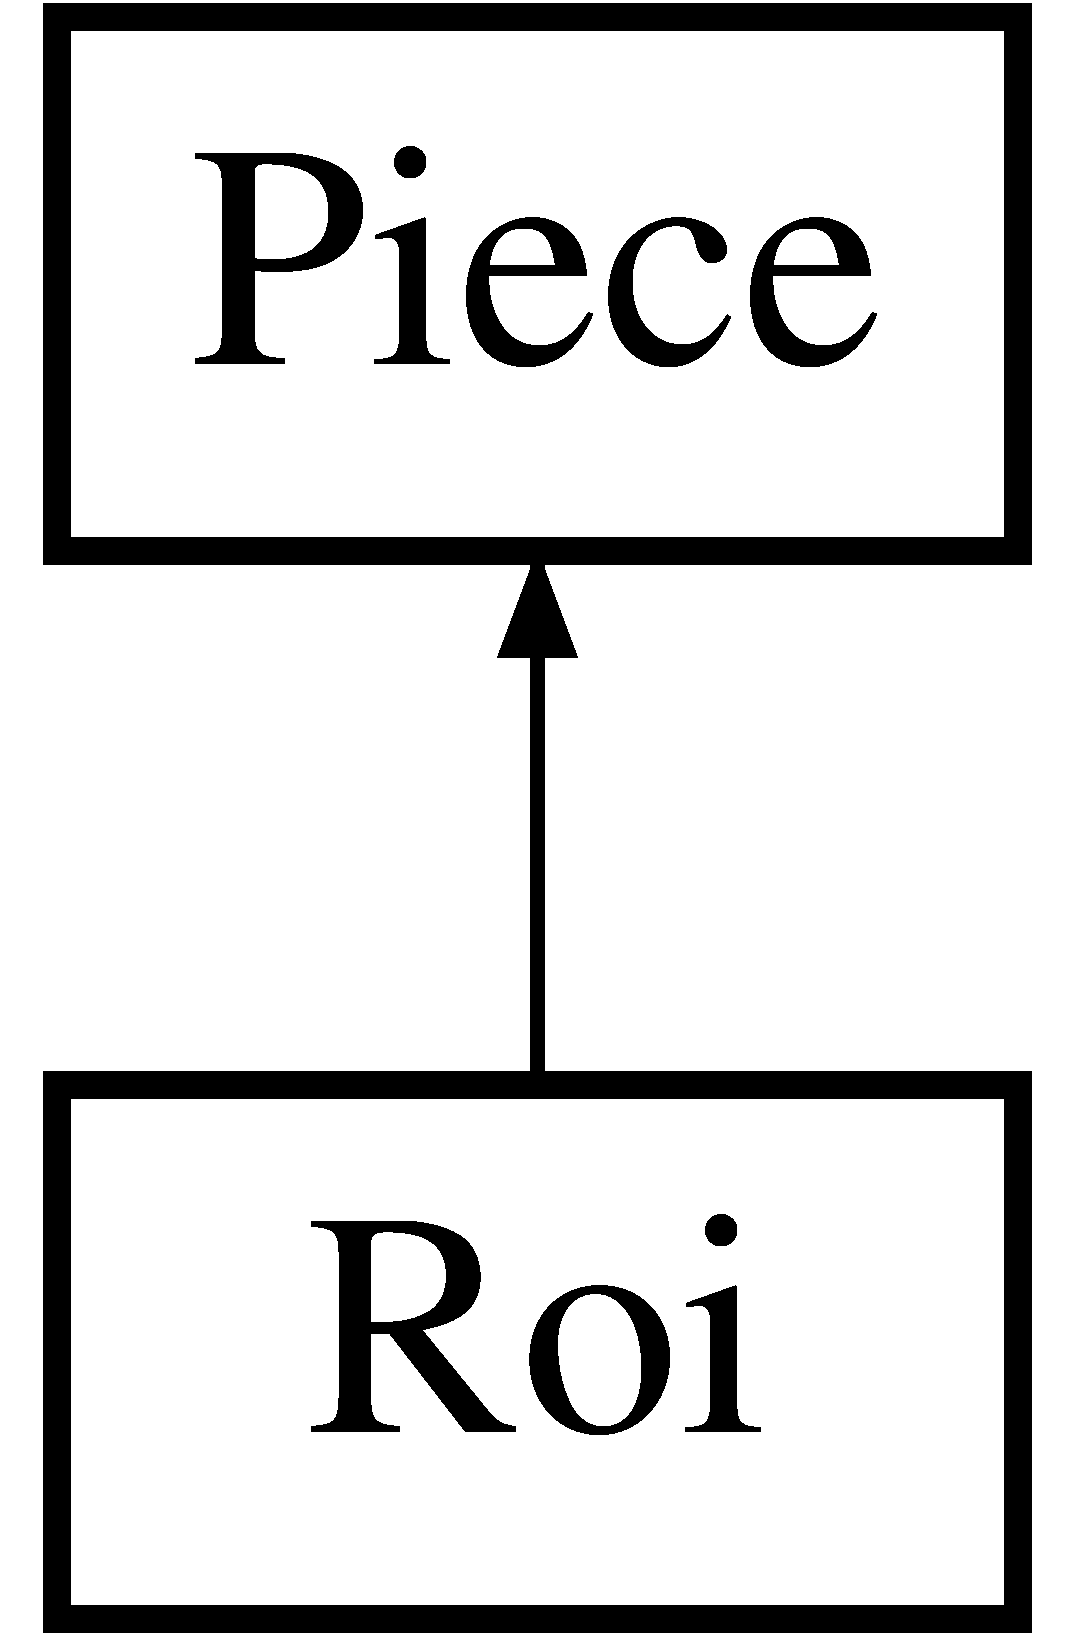
\includegraphics[height=2.000000cm]{class_roi}
\end{center}
\end{figure}
\subsection*{Public Member Functions}
\begin{DoxyCompactItemize}
\item 
{\bfseries Roi} (\hyperlink{class_case}{Case} yop)\hypertarget{class_roi_ae7848604f3ded0e548d4cc8174f124a7}{}\label{class_roi_ae7848604f3ded0e548d4cc8174f124a7}

\item 
{\bfseries Roi} (int couleur, \hyperlink{class_case}{Case} yop)\hypertarget{class_roi_a80ff4d51c676a846d0677e39d03b1dd7}{}\label{class_roi_a80ff4d51c676a846d0677e39d03b1dd7}

\item 
Array\+List$<$ \hyperlink{class_case}{Case} $>$ {\bfseries cases\+Disponibles} ()\hypertarget{class_roi_a8f5a395fb7c80f412e09de18ee52043b}{}\label{class_roi_a8f5a395fb7c80f412e09de18ee52043b}

\end{DoxyCompactItemize}
\subsection*{Additional Inherited Members}


\subsection{Detailed Description}
\begin{DoxyAuthor}{Author}
Pierrick 
\end{DoxyAuthor}


The documentation for this class was generated from the following file\+:\begin{DoxyCompactItemize}
\item 
Roi.\+java\end{DoxyCompactItemize}

\hypertarget{class_tour}{}\section{Tour Class Reference}
\label{class_tour}\index{Tour@{Tour}}
Inheritance diagram for Tour\+:\begin{figure}[H]
\begin{center}
\leavevmode
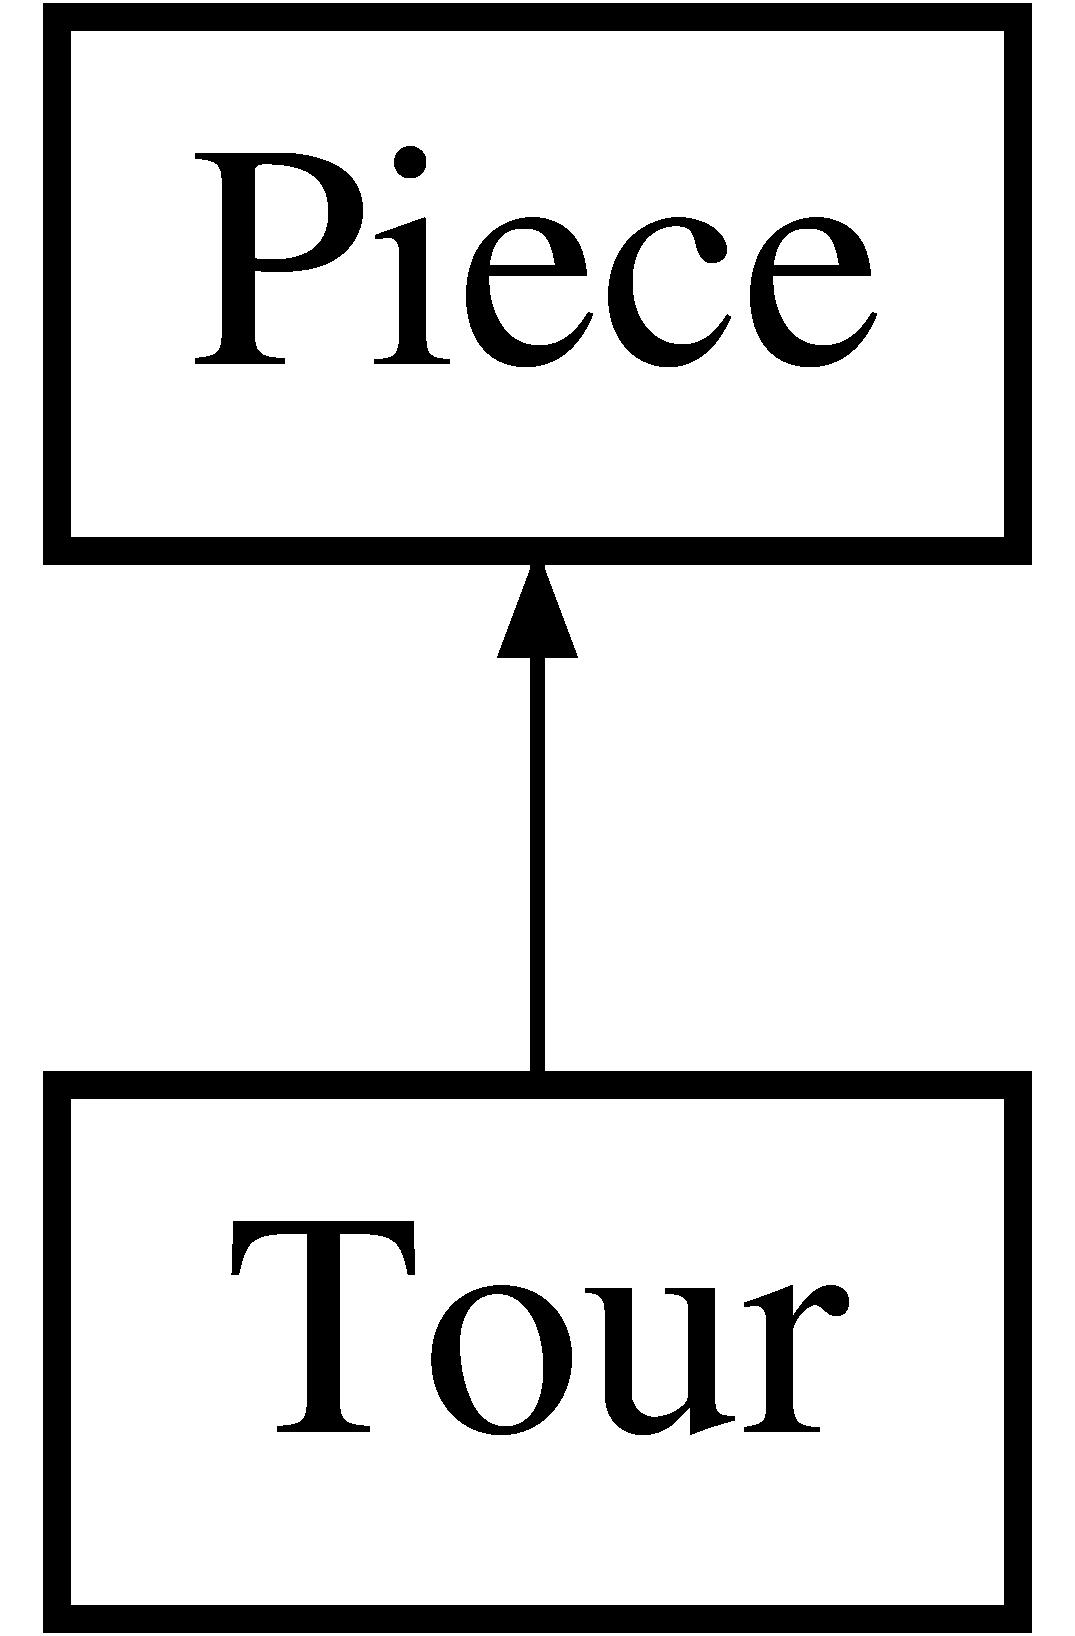
\includegraphics[height=2.000000cm]{class_tour}
\end{center}
\end{figure}
\subsection*{Public Member Functions}
\begin{DoxyCompactItemize}
\item 
{\bfseries Tour} (\hyperlink{class_case}{Case} yop)\hypertarget{class_tour_a20b303a63664f8008ead5f3ce8d6f3ac}{}\label{class_tour_a20b303a63664f8008ead5f3ce8d6f3ac}

\item 
{\bfseries Tour} (int couleur, \hyperlink{class_case}{Case} yop)\hypertarget{class_tour_ab9a41edead37945a65025a00c4d340c4}{}\label{class_tour_ab9a41edead37945a65025a00c4d340c4}

\item 
Array\+List$<$ \hyperlink{class_case}{Case} $>$ {\bfseries cases\+Disponibles} ()\hypertarget{class_tour_a0c6771d950e1432656730e34475cb855}{}\label{class_tour_a0c6771d950e1432656730e34475cb855}

\end{DoxyCompactItemize}
\subsection*{Additional Inherited Members}


The documentation for this class was generated from the following file\+:\begin{DoxyCompactItemize}
\item 
Tour.\+java\end{DoxyCompactItemize}

%--- End generated contents ---

% Index
\backmatter
\newpage
\phantomsection
\clearemptydoublepage
\addcontentsline{toc}{chapter}{Index}
\printindex

\end{document}
